\documentclass{article}
\usepackage[utf8]{inputenc}

\usepackage[spanish,es-noindentfirst]{babel}
\usepackage{graphicx}
%Code Highlighting
%\usepackage{minted}                 
\usepackage{lastpage}
\usepackage{array}


\usepackage{biblatex}

%Encabezados y pie de página
\usepackage{fancyhdr}               
\pagestyle{fancy}
\fancyhf{}
\fancyhead[L]{Práctica de la asignatura}
\fancyhead[R]{Algoritmia básica}
\fancyfoot[L]{Grado en Ingeniería Informática \\ Escuela de Ingeniería y Arquitectura}
\fancyfoot[R]{\thepage \hspace{1pt} de \pageref{LastPage}}

\renewcommand{\headrulewidth}{2pt}
\renewcommand{\footrulewidth}{1pt}

\usepackage{hyperref}
\usepackage[T1]{fontenc}
\hypersetup{
    colorlinks=true,
    linkcolor=blue,
    filecolor=magenta,      
    urlcolor=cyan,
    pdftitle={Práctica de la asignatura: El problema del viajante de comercio},                   
    bookmarks=true,
}
\urlstyle{same}

\title{Práctica de la asignatura: El problema del viajante de comercio}                            
\author{Javier Herrer Torres}      
\date{Abril 2021}                            

\begin{document}

\begin{titlepage}
    \begin{center}
        \vspace*{1cm}
            
        \Huge
        \textbf{Práctica de la asignatura}
            
        \vspace{0.5cm}
        \LARGE
        El problema del viajante de comercio
            
        \vspace{1.5cm}

        \textbf{Javier Herrer Torres} (NIP: 776609)\\
        \textbf{Javier Fuster Trallero} (NIP: 626901)

        \vfill
        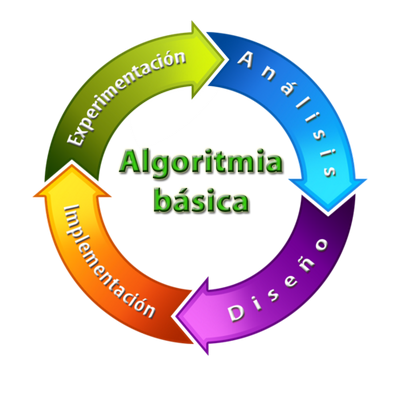
\includegraphics[width=0.25\textwidth]{../images/AB_logo_400x400}

        Algoritmia básica\\
        Grado en Ingeniería Informática\\
            
        \vspace{1.5cm}
            
        
\includegraphics[width=0.6\textwidth]{../images/eina}
            
        \vspace{1.5cm}
            
        \Large
        Escuela de Ingeniería y Arquitectura\\
        Universidad de Zaragoza\\
        Curso 2020/2021
            
    \end{center}
\end{titlepage}

\section{Metodología}

\subsection*{Fuerza bruta}
El algoritmo de \emph{fuerza bruta} para resolver el problema consiste en
intentar todas las posibilidades, es decir, calcular las longitudes de todos
los recorridos posibles, y seleccionar la de longitud mínima.
Para calcular todas las permutaciones posibles, se ha empleado el Algoritmo de
Heap.

\subsection*{Algoritmo voraz}
Se ha empleado el algoritmo de Kruscal, basado en la propiedad de los árboles de
recubrimiento mínimo. Partiendo del árbol vacío, se selecciona en cada paso la
arista de menor coste que no provoque ciclo sin requerir ninguna otra condición
sobre sus extremos. Para comprobar esta restricción, se emplea una matriz de
adyacencia de booleanos.

\subsection*{Programación dinámica}
Se trata de calcular $g(1,V \setminus \{ 1 \})$ con la función parametrizada
    $g(i,S) = min_{j \in S} \{ L_{ij} + g(j, S \setminus \{ j \}  ) \}$.

Se emplea la matriz \texttt{gtab} para almacenar los valores de $g$ calculados
para cada $S$. Esta estructura se ha implementado con un
\texttt{Map\textless{}Vertice, Map\textless{}Set\textless{}Vertice\textgreater{}, Tupla\textgreater{}\textgreater{}}
, donde \texttt{Tupla} almacena tanto el valor de $g$ como el de $J$ (para poder construir el circuito óptimo).


\subsection*{Ramificación y poda}
Se ha definido la función de estimación $\hat{c}(x)$ siguiendo los pasos de las
tranparencias del tema y el esquema algorítmico genérico. Además, se ha empleado
un montículo con prioridades (\texttt{PriorityQueue<Nodo>}) para almacenar la
frontera.


\section{Resultados}
% Resultado(s): hay que presentar los resultados, explicarlos y analizarlos.
Los siguientes resultados (cuadro \ref{tab:tiempos} y la figura \ref{graph:tiempos})
se han obtenido con matrices generadas aleatoriamente con un cierto número de
vértices. Estas matrices representan grafos dirigidos.

\begin{table}[h]
    \centering
    \begin{tabular}{r|rrrr}
        \hline
        \multicolumn{1}{l}{\textbf{Vértices}} & \multicolumn{1}{l}{\textbf{FB}} & \multicolumn{1}{l}{\textbf{AV}} & \multicolumn{1}{l}{\textbf{PD}} & \multicolumn{1}{l}{\textbf{RyP}} \\ \hline \hline
        7                                     & 321                             & 15                              & 104                             & 17                               \\
        8                                     & 1292                            & 14                              & 180                             & 25                               \\
        9                                     & 6346                            & 13                              & 368                             & 42                               \\
        10                                    & 96438                           & 15                              & 516                             & 98                               \\
        11                                    &                                 & 14                              & 1081                            & 62                               \\
        12                                    &                                 & 17                              & 1800                            & 61                               \\
        13                                    &                                 & 19                              & 3641                            & 82                               \\
        14                                    &                                 & 17                              & 10194                           & 53                               \\
        15                                    &                                 & 18                              & 35922                           & 158                              \\
        16                                    &                                 & 20                              & 120832                          & 164                              \\
        17                                    &                                 & 18                              & 447403                          & 72                               \\
        18                                    &                                 & 19                              & 1722253                         & 145                              \\
        19                                    &                                 & 19                              & 6558672                         & 82                               \\
        20                                    &                                 & 20                              &                                 & 131                              \\
        21                                    &                                 & 19                              &                                 & 340                              \\
        22                                    &                                 & 23                              &                                 & 241                              \\
        23                                    &                                 & 22                              &                                 & 699                              \\
        24                                    &                                 & 21                              &                                 & 6211                             \\
        25                                    &                                 & 22                              &                                 & 8100                             \\
        26                                    &                                 & 23                              &                                 & 11213                            \\
        27                                    &                                 & 22                              &                                 & 16770                            \\
        28                                    &                                 & 28                              &                                 & 28384                            \\
        29                                    &                                 & 27                              &                                 & 18160                            \\
        30                                    &                                 & 25                              &                                 &                                  \\
        50                                    &                                 & 71                              &                                 &                                  \\
        100                                   &                                 & 147                             &                                 &                                  \\
        500                                   &                                 & 1439                            &                                 &                                  \\
        1000                                  &                                 & 3445                            &                                 &                                  \\ \hline
    \end{tabular}
    \caption{Tiempos de ejecución en ms.}
    \label{tab:tiempos}
\end{table}

\begin{figure}[h]
    \centering
    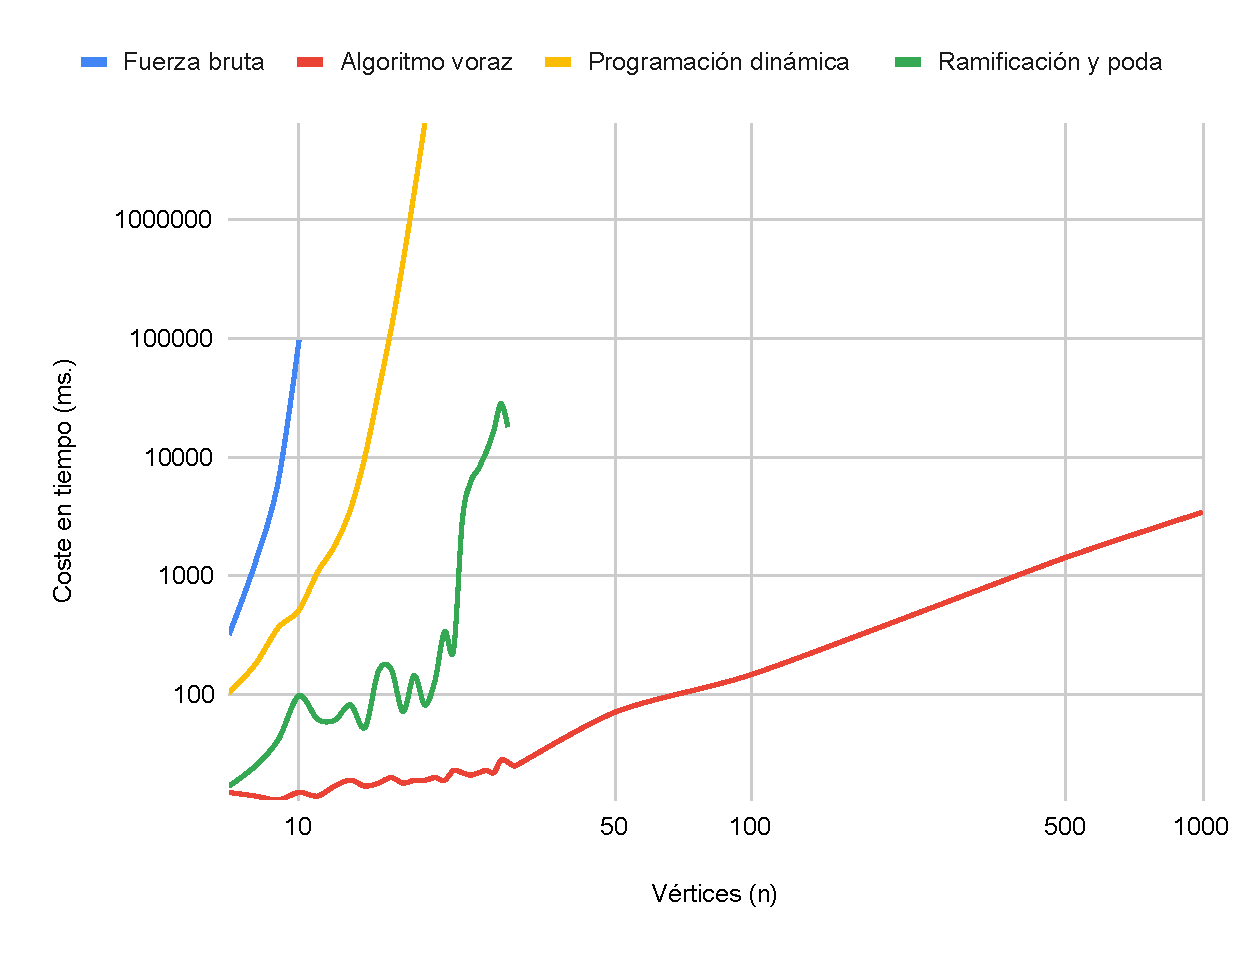
\includegraphics[width=0.9\textwidth]{../images/chart}
    \caption{Gráfico de costes temporales}
    \label{graph:tiempos}
\end{figure}

Además, en el cuadro \ref{tab:ficheros-proporcionados} se han incluido los
resultados obtenidos para los ficheros proporcionados en los que ha sido posible
ejecutar los algoritmos.

\begin{table}[h]
    \centering
    \begin{tabular}{c|rrr}
        \hline
        \multicolumn{1}{l}{\textbf{Fichero}} & \multicolumn{1}{l}{\textbf{AV}} & \multicolumn{1}{l}{\textbf{PD}} & \multicolumn{1}{l}{\textbf{RyD}} \\ \hline \hline
        a4                                   & 13                              & 12                              & 13                               \\
        a11                                  & 14                              & 1162                            & 72                               \\
        a15                                  & 19                              & 40531                           & 179                              \\
        a16                                  & 21                              & 136522                          & 151
    \end{tabular}
    \caption{Resultados para los ficheros proporcionados}
    \label{tab:ficheros-proporcionados}
\end{table}


\section{Conclusiones}
% Conclusiones: es lo último que se lee, por tanto es una sección muy importante que se debe utilizar para remarcar los mensajes que queremos que el lector reciba. Por ejemplo, si estamos evaluando un producto podemos enfatizar sus puntos fuertes y sus puntos débiles, y señalar posibilidades de mejora.
    El \textbf{algoritmo de fuerza} para resolver el problema consiste en intentar todas
    las posibilidades. Obviamente, el coste crece exponencialmente con el número
    de puntos a visitar.

    El \textbf{algoritmo voraz} tiene el mejor coste temporal, pero debe destacarse que
    \emph{tiene la posibilidad, pero no la certeza, de encontrar la solución óptima}.
    De hecho, en la mayoría de casos no la encuentra aunque el coste pueda
    aproximarse al óptimo.

%Programación dinámica

    \textbf{Programación dinámica} mejora a fuerza bruta pasando de un tiempo $\Omega (n!)$
    a $\Theta (n^2 2^n)$, es decir, \emph{pasando de un coste temporal
    factorial a exponencial}. Pero, a cambio, el coste en espacio es de $\Omega (n 2^n)$
    resultante de almacenar la matriz \texttt{gtab}. A partir de 19 vértices,
    el tamaño de esta matriz crece generando un \texttt{java.lang.OutOfMemoryError: Java heap space}.


    En el algoritmo de \textbf{Ramificación y poda}, el coste del caso peor de la solución;
    pese a ser teóricamente el mismo que en programación dinámica, $\Theta (n^2 2^n)$;
    se observa una clara diferencia en la práctica. Pudiendo resolver problemas de hasta
    10 vértices más. A partir de 29 vértices, el tamaño de la frontera crece
    generando un \texttt{java.lang.OutOfMemoryError: Java heap space}.
    Además, se ha apreciado que en este algoritmo existe una
    gran variabilidad en el coste temporal para distintas matrices con mismo
    número de vértices, esto se debe a la función de poda.



%\printbibliography
%Normalmente al final se incluyen referencias, bibliografía, índice de expresiones técnicas y anexos.

\end{document}
